% !TEX root = ../thesis.tex

\chapter{Two-Qubit Gates for the Soft \zps Qubit}\label{chp:zp_2q_gates}

This chapter is adapted from Ref.~\cite{liu2026zp2q}, written with Zhenxing Liu and Joshua Combes.

\section{Introduction}
The transmon and fluxonium are the workhorses of superconducting quantum computing.
They combine relatively simple fabrication with high performance ~\cite{kochChargeinsensitiveQubitDesign2007b,manucharyanFluxoniumSingleCooperPair2009a,nguyen_high-coherence_2019,aruteQuantumSupremacyUsing2019a}.
Their coherence times, however, are limited by a trade-off between relaxation and dephasing.
The transmon suppresses charge-noise dephasing but is susceptible to energy relaxation.
Heavy fluxonium is comparatively robust against relaxation but more sensitive to flux-noise dephasing.
The standard approach to overcome this issue is to use error correction.
The relaxation/dephasing trade-off is generic to single-mode superconducting qubits, which cannot be strongly protected against both relaxation and dephasing~\cite{gyenisMovingTransmonNoiseProtected2021b}.

Multimode circuits offer an alternative route beyond this limitation.
They can realize \textit{protected qubits}~\cite{gyenisMovingTransmonNoiseProtected2021b} that are resistant to both energy relaxation and dephasing, and thus can lower error rates.
However, this protection comes at the cost of increased circuit and fabrication complexity.
Replacing transmons and fluxoniums with such protected qubits could reduce the error-correction overhead for large-scale quantum computation~\cite{eisert2025}.

Among protected-qubit proposals, the \zps qubit is one of the most widely studied~\cite{kitaev_protected_2006}.
Since its introduction~\cite{kitaev_protected_2006,brooks2013}, studies have examined disorder~\cite{Dempster2014understanding}, coherence~\cite{groszkowski2018}, readout and control~\cite{paolo_control_2019,Gyenis_zero_pi_2021a}, and tunable circuit designs~\cite{shenTheoreticalAnalysisProtected,smithSuperconductingCircuitProtected2020b,egusquiza2021,guo2022,rajpoot2022tunable}.
The first experimental realization operated in a partially protected ``soft'' regime~\cite{Gyenis_zero_pi_2021a}, with exponential protection against relaxation but only first-order protection against dephasing.
Full protection requires large inductances and small stray capacitances, which pose major fabrication challenges.
Although recent advances have moved experimental parameters closer to the ideal regime~\cite{KimAPS2024,kim2025protected}, near-term \zps devices are likely to remain soft, with steadily increasing protection.

Long-lived qubits alone are not enough for quantum computation.
Universal control also requires high-fidelity single- and two-qubit gates.
Fully protected gates are possible~\cite{kolesnikowProtectedPhaseGate2026} but are difficult to realize experimentally.
Near-term \zps devices will likely rely on unprotected gates that do not preserve the qubit’s protection.
Indeed, an unprotected single-qubit gate has been experimentally demonstrated in the soft 0-$\pi$ regime~\cite{Gyenis_zero_pi_2021a}.
Sufficiently fast and high-fidelity gates could help make these approaches more viable for larger-scale quantum computation.

This leaves an important gap.
To our knowledge, no microwave-activated, unprotected two-qubit gate has been proposed for experimentally relevant soft \zps devices.
Such gates are challenging because coupling two \zps qubits requires multi-node interactions, the computational states depend on external flux, and matrix elements are suppressed within the logical subspace due to protection.
As a result, many gate mechanisms used in transmon architectures do not directly apply.

\begin{figure}[htbp]
\centering
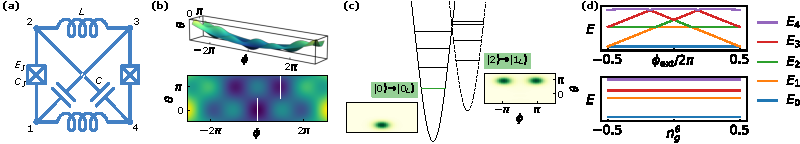
\includegraphics[width=\textwidth]{chapter-4-zero-pi/figs/circuit.pdf}
\caption[Overview of the soft \zps qubit.]{An overview of a soft \zps qubit.
(a) Circuit diagram.
The circuit consists of two capacitors with capacitance $C$, two inductors with inductance $L$, and two Josephson junctions with Josephson energy $E_{J}$ and junction capacitance $C_J$.
Each circuit node, labeled by $i\in\{1,2,3,4\}$, is associated with a flux variable $\varphi_i$ shown in \cref{zp:eq:zp_transform}.
(b) Three-dimensional surface plot and two-dimensional map of potential energy $V(\theta, \phi)$ at $\phiext=0$, with parameters of qubit 1 from \cref{zp:tab:parameter_zp}.
(c) Lowest ten eigenvalues (horizontal lines) are plotted in the double-well potential with a solid-line well ($\phi=0$) and a dashed-line well ($\phi=\pi$), corresponding to the solid and dashed white lines in (b).
The two logical states $\ket{0_L} = \ket{0}$ and $\ket{1_L}=\ket{2}$ are highlighted in green and are strongly localized inside the two valleys.
(d) Energy spectrum of the lowest five eigenvalues versus external flux $\phiext/2\pi$ in flux quanta at $n_g^{\theta}=0$ in the top panel, and versus offset-charge $n_g^{\theta}$ at $\phiext=0$ in the bottom panel.
}\label{zp:fig:circuit_potential}
\end{figure}

In this chapter, we address this gap by proposing an unprotected controlled-$Z$ (CZ) gate for capacitively coupled soft \zps qubits.
Since accurately simulating two coupled \zps circuits requires a large Hilbert space, we focus on the idealized zero-disorder limit.
This assumption substantially reduces the required Hilbert-space dimension but eliminates an important source of device imperfections.
The resulting gate performance should therefore be interpreted as a best-case bound for realistic devices.

The organization of this chapter is as follows.
In \cref{zp:sec:basics}, we introduce the basics of a single \zps qubit.
In \cref{zp:sec:1q}, we optimize single-qubit $X$ gates using a voltage drive that capacitively couples to the $\phi$ or $\theta$ mode.
In \cref{zp:sec:coupling}, we introduce a capacitive coupling scheme between two \zps circuits.
In \cref{zp:sec:cz}, we introduce the CZ gate.
In \cref{zp:sec:fidelity_2q}, we develop a two-qubit noise model and evaluate the performance of the CZ gate in the presence of noise.
Finally, in \cref{zp:sec:conc}, we conclude with open questions.

\section{Basics of the \texorpdfstring{\zp}{zero pi} Qubit}\label{zp:sec:basics}
In this section, we introduce the basics of the \zps qubit.
Readers interested in more details should consult references~\cite{Dempster2014understanding,paolo_control_2019,groszkowski2018,Gyenis_zero_pi_2021a}.
The four-node \zps circuit is built using pairs of capacitors, inductors, and Josephson junctions.
As shown in \cref{zp:fig:circuit_potential}(a), each circuit node is connected to one element of each type.

Because the \zps circuit contains multiple modes, the node flux variables $\varphi_i$ are not the easiest way to understand the circuit.
To obtain variables that are easier to interpret, we use the variable transformation from Ref.~\cite{Dempster2014understanding}
\begin{align}\label{zp:eq:zp_transform}
\left(\begin{array}{c}
{\theta} \\
{\phi} \\
{\zeta} \\
{\Sigma} \\
\end{array}\right)=\frac{1}{2}\left(\begin{array}{rrrr}
-1 & \phantom{-}1 & 1  & -1 \\
-1 & 1 & -1  & 1 \\
1 & 1 & -1  & -1 \\
1 & 1 & 1  & 1 \\
\end{array}\right)\left(\begin{array}{c}
\varphi_1 \\
\varphi_2 \\
\varphi_3 \\
\varphi_4 \\
\end{array}\right) \,.
\end{align}
The $\theta$ mode is transmon-like, as it depends on the phase differences across junctions and capacitors.
Similarly, the $\phi$ mode is fluxonium-like, as it depends on the phase differences across junctions and inductors.

We make the simplifying assumption that all the capacitances, inductances, and junctions are the same (zero-disorder).
Under this assumption, the LC-like $\zeta$ mode decouples exactly from other modes (and can be ignored), as can the cyclic $\Sigma$ mode~\cite{taylor2005classical}.
The energy stored in any individual circuit element is thus parameterized by $E_C = e^2/2C$, $E_L = \phi_0^2/ L$, and $E_J = I_c \phi_0$, where $\phi_0 = \hbar /2e$ is the reduced flux quantum, $I_c$ is the critical current of the Josephson junction, and $C$ and $L$ are the capacitance and inductance, respectively.
Because the zero-disorder assumption is not experimentally realistic, our work represents an upper bound on the performance for more realistic devices.

In the zero-disorder limit, we consider only the $\theta$ and $\phi$ modes.
Circuit quantization yields generalized flux operators  $\hat{\theta}$ and $\hat{\phi}$ and conjugate charge operators $\hat{n}_{\theta}$ and $\hat{n}_{\phi}$ such that, e.g., $[\hat{\phi}, \hat{n}_\phi] = i$ \cite{Dempster2014understanding}.
For the remainder of the chapter, we will omit hats on operators for simplicity.
We also introduce an offset charge $n_g^{\theta}$ and an external flux bias $\phi_{\rm ext}$.
Using these operators, the two-mode quantum Hamiltonian for the \zps circuit is expressed as
\begin{align} \label{zp:eq:zp Hamiltonian}
\begin{split}
    H_{0\text{-}\pi} =&\, 4E_C^\theta ({n}_{\theta}-n_g^{\theta})^2 + 4E_C^\phi {n}_{\phi}^2 \\
    &+ E_L {\phi} ^2  - 2 E_J \cos{\theta} \cos\left({\phi} -\frac{\phiext}{2}\right) \,,
\end{split}
\end{align}
where $\phi_{\rm ext} = \Phi_{\rm ext}/\phi_0$.
The charging energies of the $\theta$ and $\phi$ modes are
\begin{align}
    E_C^\theta = \frac{e^2}{2C_\theta} \quad \text{and} \quad
    E_C^\phi  = \frac{e^2}{2C_\phi}  \, ,
\end{align}
where $C_\theta =2C +2C_J +C_0$ and $C_\phi = 2C_J +C_0$.
Here $C_J$ is the junction capacitance and $C_0$ is the capacitance between the nodes and ground [not shown in \cref{zp:fig:circuit_potential}(a)].

We now explain why the \zps is a protected qubit.
Protection against energy relaxation is achieved by choosing logical states with disjoint support \cite{gyenisMovingTransmonNoiseProtected2021b}.
Any charge matrix elements (and corresponding decay rates) between them are thus suppressed.
The selection of the computational states of the \zps circuit can thus be understood from the potential energy $V(\theta, \phi) = E_L \phi^2 - 2 E_J \cos\theta \cos\phi$, corresponding to the second line of \cref{zp:eq:zp Hamiltonian}, evaluated at the working point $\phiext = 0$.
In \cref{zp:fig:circuit_potential}(b) we plot $V(\theta, \phi)$ using experimentally realized parameters of the \zps qubit.
The exact values are shown as qubit 1 in \cref{zp:tab:parameter_zp}.
As seen in \cref{zp:fig:circuit_potential}(b)--(c), the logical states of the soft \zp, $\ket{0_L}=\ket{0}$ and $\ket{1_L}=\ket{2}$, are chosen to be the lowest states in the $\phi=0$ and $\phi=\pi$ valleys.
To ensure disjoint support, the effective barrier height between the two valleys ($\approx 4E_J$) must be much larger than the qubit frequency ($\approx E_L \pi^2$) and the kinetic energy ($E_C^{\theta}$) along the $\theta$ direction, i.e., $E_J\gg E_L, E_C^{\theta}$.
Note that the first excited state is in the $\phi=0$ valley, so selecting $\ket{1_L} = \ket{1}$ would not yield a protected qubit.

\begin{table}[htbp]
\centering
\setlength{\tabcolsep}{3.5pt}
\begin{tabular}{cccccccc}
\toprule
Q & $E_J$ & $E_L$ & $E_C^{\theta}$ & $E_C^{\phi}$ & $E_{C_c}$ & $E_{C_0}$ & $g_{\theta}$ \rule{0pt}{2.8ex} \\[1pt] \midrule
\rule{0pt}{2.4ex} 1   & 6.013  & \multirow{2}{*}{0.377}  & \multirow{2}{*}{0.092}  & \multirow{2}{*}{1.14} & \multirow{2}{*}{1.0} & \multirow{2}{*}{1.491} &  \multirow{2}{*}{0.031}    \\
2   & 5.412  &  &   &  &   & &    \\ \bottomrule
\end{tabular}
\caption[Soft \zps qubit parameters.]{
Parameters for two soft \zps qubits in units of $h \cdot \text{GHz}$.
Qubit 1 is the experimentally realized soft \zps from \cite{Gyenis_zero_pi_2021a}, and qubit 2 is an otherwise identical system with $E_J$ reduced by 10\%.
We consider qubit 1 for all single-qubit studies.
}\label{zp:tab:parameter_zp}
\end{table}

The dephasing protection of the \zps is realized by suppressing the charge and flux dispersions.
In \cref{zp:fig:circuit_potential}(d) we plot the eigenvalues of \cref{zp:eq:zp Hamiltonian} as a function of the offset charge $n_g^\theta$ and external flux $\phi_{\rm ext}$.
The charge dispersion is exponentially suppressed via a large ratio of $E_J/ E_C^{\theta}$, following the same mechanism as the transmon qubit \cite{kochChargeinsensitiveQubitDesign2007b}.
As for the flux dispersion, the symmetric and antisymmetric states in the two local minima of the $\theta=\pi$ valley give a hyperbolic dispersion as a function of $\phi_{\rm ext}$, so first-order protection can be achieved at $\phi_{\rm ext}=0$.
Further flattening of the flux dispersion requires delocalization of wavefunctions along the $\phi$ direction, which entails larger kinetic energy $E_C^\phi$.
To summarize, an ideal hard \zps qubit requires $E_L,E_C^\theta \ll E_J,E_C^\phi$ in order to achieve full protection against both energy relaxation noise and pure dephasing noise from flux and charge fluctuations.

\begin{figure}[htbp]
\centering
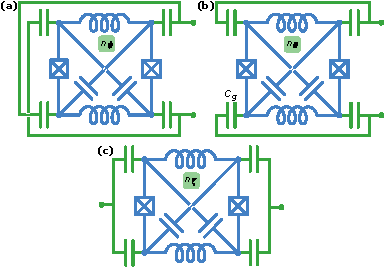
\includegraphics[width=\colfigwidth]{chapter-4-zero-pi/figs/circuit_1qubit.pdf}
\caption[Electrical connections for coupling to the \zps modes.]{Electrical connections required to couple to the $\phi$, $\theta$, and $\zeta$ modes of the \zps qubit~\cite{paolo_control_2019}.
The \zps and coupling circuit are shown in blue and green respectively.
A microwave source is connected across the two green nodes to drive a specific mode.
}
\label{zp:fig:circuit_3modes}
\end{figure}

To control the \zps qubit, we must couple to it.
We consider only capacitive coupling, as inductive connections break the periodicity of the qubit potential -- except in the $L \to \infty$ limit~\cite{paolo_control_2019}.
We are primarily interested in coupling to the $\theta$ and $\phi$ modes, but coupling to the $\zeta$ mode may be necessary to cool the system and suppress photon shot noise \cite{paolo_control_2019}.
To selectively couple to a single mode of the \zps qubit, individual connections to all four circuit nodes are required (see \cref{zp:fig:circuit_3modes}), which is difficult to achieve in practice.
Recent work has aimed to enable access to all four nodes~\cite{KimAPS2024,kim2025protected} through the use of parallel-plate instead of interdigitated capacitors.
In this paper, we assume that each node of the \zps circuit can be electrically accessed and that the individual modes can be addressed.

In the experimental implementation of \zp, the authors use a higher non-logical state $\ket{9}$ to transform the qubit into an effective $\Lambda$ system and transfer population between the two logical states~\cite{Gyenis_zero_pi_2021a}.
Since certain nodes of the circuit were inaccessible, it was not possible to employ the coupling schemes in \cref{zp:fig:circuit_3modes}.
The experimental device induces transitions primarily by coupling to the $n_\phi$ operator, with residual coupling to $n_\theta$.
This scheme is known to have problems, such as leakage into even higher energy levels~\cite{PremkumarAPS2023,premkumar2023hamiltonian}.
We will discuss these limitations in detail in the next section.
There are several alternative proposals for single-qubit gates for the \zps qubit, but they are primarily focused on the more strongly protected ``hard'' \zps regime \cite{paolo_control_2019,kolesnikowProtectedPhaseGate2026}.

\section{Single-Qubit \texorpdfstring{$X$}{X} Gates}
\label{zp:sec:1q}
In this section, we investigate the limitations of unprotected single-qubit $X$ gates in the soft \zps qubit that use population transfer via a non-logical state.
Assuming the capacitive coupling shown in \cref{zp:fig:circuit_3modes}, we consider driving the $\phi$ and $\theta$ modes individually.
Because both gates are driven through the charge operators, we refer to them as the $n_\phi$-driven and $n_\theta$-driven gates.
We show that shorter, higher-fidelity operations are achieved by driving $n_\theta$, which is consistent with previous studies \cite{abdelhafez2020universal}.

\subsection{Driven Hamiltonian}\label{zp:sec:1q_drive}
All single-qubit gate schemes in this work are implemented using two-tone drives.
The full Hamiltonian of the qubit with drive can be expressed as
\begin{align}\label{zp:eq:H_total_and_drive_xgate}
    H_{\rm tot} = H_{0\text{-}\pi} + H_{\rm drive},
\end{align}
where the parameters for $H_{0\text{-}\pi}$ come from the first qubit in \cref{zp:tab:parameter_zp}.
The microwave drives are parametrized as
\begin{align} \label{zp:eq:zp_H_drive}
H_{\rm drive} = \sum_i {A_if(t)\cos{(\omega_{di} t)} n_{\rm op} } \, ,
\end{align}
where $A_i$ is the drive amplitude, $\omega_{di}$ is the drive frequency, and  $n_{\rm op} \in \left\{n_{\rm \theta}, n_{\rm \phi}\right\}$ is a charge operator.
For a pulse of length $t_g$, we choose $f(t)$ to be a Gaussian drive envelope\footnote{Because a Gaussian $g(t) = \exp[-(t-t_g/2)^2 / 2(t_g/4)^2] $ has $\mu=t_g/2$ and $\sigma = t_g/4$, the envelope $f(t) = \exp[-8t(t-t_g) / t_g^2] - 1 = e^2 (g(t) - g(0)) = e^2 (g(t) - g(t_g))$ has a $4\sigma$ width.
Note that $f(t)$ has a maximum of $e^2-1$, so the maximum amplitude of the drive is $A_i f(t)= A_i(e^2-1)$.}
\begin{align} \label{zp:eq:gauss_envelope}
f(t) =
\begin{cases}
  0, &  t < 0\ \text{or}\  t > t_g \\
  e^{-8t(t-t_g)/t_g^2}-1 , &  0 \leq t \leq t_g
\end{cases} ~.
\end{align}

Below we identify an effective $\Lambda$ system for each charge operator by finding an intermediate state $\ket{\lambda}$ with achievable transitions $\ket{0_L} \leftrightarrow \ket{\lambda}$ and $\ket{1_L} \leftrightarrow \ket{\lambda}$.
The transition frequency between levels $\ket{a}$ and $\ket{b}$ is denoted as $\omega_{a\text{-}b}$.
Each transition is driven by a separate pulse with amplitude $A_i$ and drive frequency
\begin{equation}
  \omega_{di} =  \omega_{i\text{-} \lambda}+\delta_{i}\, ,
\end{equation}
where $i \in \{ 0_L, 1_L\}$ and $\delta_{i}$ is the detuning.
Similarly, we denote the charge matrix element between levels $\ket{a}$ and $\ket{b}$ as
\begin{equation}
    n_{\rm op}^{a\text{-}b} = \left|\bra{a} n_{\rm op} \ket{b}\right|.
\end{equation}

\subsection{\texorpdfstring{$X$}{X} gate by driving \texorpdfstring{$n_\phi$}{phi} } \label{zp:sec:1q_phi}

We first consider directly coupling to the $\phi$ mode.
The $n_\phi$ operator induces an effective $\Lambda$ system involving $\ket{0}$, $\ket{2}$, and $\ket{9}$, as illustrated in \cref{zp:fig:xgate_phi}(a).
The colored arrows denote the target transitions.
Numerous additional transitions give rise to significant leakage channels.
Black dashed arrows denote ``level-1'' leakage transitions that go from states in the $\Lambda$ system to level-1 states.
Gray dashed arrows show level-2 leakage (from level-1 to level-2 states), and gray dotted lines indicate higher-level leakage.
We use these connections to infer leakage pathways.
For example, state $\ket{37}$ couples to states ($\ket{9},\ket{10}$), which in turn couple back to the computational space ($\ket{0},\ket{2}$).

\Cref{zp:fig:xgate_phi}(b) shows the population of several levels during an $X$ gate of fidelity 99.659\% with gate time $t_g=180.0$ ns.
The populations of logical states and leakage states are plotted separately, with $\ket{9}$ shown in both subplots for scale.
We show only the most-populated leakage states, while the total population of all remaining states is grouped into the category “other.” Multiple leakage states have comparable population to state $\ket{9}$ during gate operation, with the top three being $\ket{10}$, $\ket{19}$, and $\ket{33}$.

To identify the associated leakage transitions, we plot charge matrix elements $n_\phi^{i \text{-} j}$ for these states as a function of transition frequency $\omega_{i \text{-} j}$ in \cref{zp:fig:xgate_phi}(c).
The two transitions forming the $\Lambda$ system are shown in blue and orange, with corresponding drive frequencies marked by red arrows.
These optimized drives are off-resonant due to the presence of nearby transitions.
The dashed lines indicate levels of leakage using the same color scheme as \cref{zp:fig:xgate_phi}(a).
The dominant level-1 leakage transitions appear to be $\ket{0}$-$\ket{10}$, $\ket{2}$-$\ket{19}$, and $\ket{9}$-$\ket{33}$.
Importantly, the $\ket{10} \leftrightarrow \ket{37}$ transition is nearly resonant with the $\ket{0} \leftrightarrow \ket{9}$ transition but has a much larger matrix element.
Leakage to such a transition can be reduced by limiting population in the intermediate and level-1 leakage states.
Due to frequency crowding, the drive strength must be kept small compared to the detuning from neighboring transitions to suppress leakage, resulting in long gate times.

\begin{figure}[htbp]
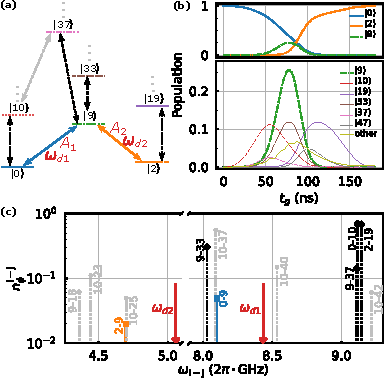
\includegraphics[width=\colfigwidth]{chapter-4-zero-pi/figs/xgate_phi.pdf}
\centering
\caption[Optimized $X$ gate driving $n_\phi$.]{
Numerically optimized $X$ gate by driving $n_\phi$, with $F= 99.659\%$ and $t_g=180.0~\mathrm{ns}$.
(a) Energy level diagram.
The desired transitions, $\ket{0}$-$\ket{9}$ and $\ket{2}$-$\ket{9}$, are shown with blue and orange arrows.
These transitions are driven with amplitudes $A_i$ and frequencies $\omega_{di}$ for $i\in\{1,2\}$.
Leakage pathways are denoted with dashed arrows.
Black arrows represent ``level-1'' leakage transitions, while gray arrows represent ``level-2'' leakage transitions that involve level-1 states.
(b) Population transfer.
``other'' denotes the total population of states that are not explicitly shown.
(c) Charge matrix elements $n_\phi^{i \text{-} j}$ versus transition frequency $\omega_{i \text{-} j}$.
The line colors and styles match those in (a).
The desired transitions have $\omega_{0\text{-}9}/2\pi=8.100\ {\rm GHz}$ and $\omega_{2\text{-}9}/2\pi=4.697\ {\rm GHz}$, with $n_{\phi}^{0\text{-}9}=0.049$ and $n_{\phi}^{2\text{-}9}=0.020$.
Simulations use the lowest 1000 levels; see \cref{zp:app:1Qgate_simulation} and our open-source GitHub repository \cite{zp2q_repo} for numerical implementation details.
Pulse parameters can be found in \cref{zp:tab:xgate_parameters}.
}\label{zp:fig:xgate_phi}
\end{figure}

\subsection{\texorpdfstring{$X$}{X} gate by driving \texorpdfstring{$n_\theta$}{theta}}  \label{zp:sec:1q_theta}
\begin{figure}[htbp]
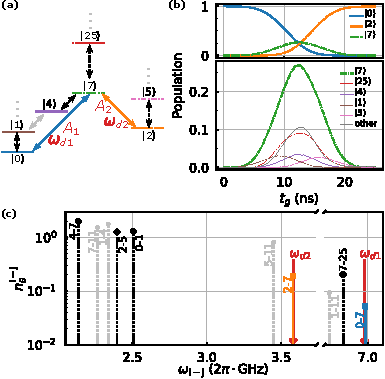
\includegraphics[width=\colfigwidth]{chapter-4-zero-pi/figs/xgate_theta.pdf}
\centering
\caption[Optimized $X$ gate driving $n_\theta$.]{
Numerically optimized $X$ gate by driving $n_\theta$, with $F=99.758\%$ and gate time $t_g$ = 25.0 ns.
(a) Energy level diagram.
Leakage pathways are denoted with dashed arrows.
Black arrows show ``level-1'' leakage transitions involving an intentionally populated state ($\ket{0}$, $\ket{2}$, or $\ket{7}$).
(b) Population transfer.
``other'' includes the total population of all states not explicitly shown.
(c) Charge matrix elements $n_\theta^{i \text{-} j}$ versus transition frequency $\omega_{i \text{-} j}$.
The two Raman transition frequencies are $\omega_{0\text{-}7}/2\pi=6.983\ {\rm GHz}$ and $\omega_{2\text{-}7}/2\pi=3.580\ {\rm GHz}$, with $n_{\theta}^{0\text{-}7}=0.052$ and $n_{\theta}^{2\text{-}7}=0.191$.
Pulse parameters can be found in \cref{zp:tab:xgate_parameters}.
}\label{zp:fig:xgate_theta}
\end{figure}

Now we perform an $X$ gate by driving the $\theta$ mode.
The $n_\theta$ operator induces a $\Lambda$-like system involving $\ket{0}$, $\ket{2}$, and $\ket{7}$.
\Cref{zp:fig:xgate_theta}(b) shows the population transfer for an $X$ gate with a fidelity of 99.758\% and gate time $t_g$ = 25.0 ns.
The two drive frequencies $\omega_{d1}$ and $\omega_{d2}$ are indicated by red arrows in \cref{zp:fig:xgate_theta}(c).
Unlike the $n_\phi$ case, there is a single most prominent leakage state $\ket{25}$, which is populated through the $\ket{7}$-$\ket{25}$ transition.
The next most prominent leakage states are $ \ket{1}$, $\ket{4}$, and $\ket{5}$.
The transitions that populate these states are strongly detuned, but the relevant matrix elements are roughly an order of magnitude larger than those in the $\Lambda$ system, leading to significant population transfer.
Nonetheless, there is substantially less leakage overall when driving the $\theta$ mode compared to driving the $\phi$ mode.

We can also compare our results with those of \citet{abdelhafez2020universal}.
In that work, the authors use optimal control to design an $X$ gate for the \zps qubit in a harder parameter regime (larger $E_J, E_C^\phi$ and smaller $E_L,E_C^\theta$).
The authors drive $n_\theta$ with an amplitude of 1.5 GHz $\approx 238\times 2\pi$ MHz, which is comparable to the drive amplitude used in our gate; see \cref{zp:tab:xgate_parameters}.
For a gate time $t_g=$ 60 ns, they achieve an $X$ gate with 98.6\% coherent fidelity.\footnote{This is also consistent with \citet{paolo_control_2019} when the fidelity and gate time are extracted from its results.
That work uses the same parameters as Ref.~\cite{abdelhafez2020universal}.}
Although this indicates lower performance than for our $X$ gate, slower gates are expected in this more strongly protected \zps parameter regime.
Indeed, when we simulate a Raman-style $X$ gate in the same parameter regime, we see comparable gate fidelities for this gate time.

\subsection{Single-Qubit Noise Model}\label{zp:sec:noise_1q}
To study the effects of noise on these gates, we use a Lindblad master equation to phenomenologically include energy relaxation and dephasing.
The evolution of the state matrix is given by
\begin{align} \label{zp:eq:master_eq}
\frac{d\rho}{dt} = -\frac{i}{\hbar}[H, \rho] + \sum_{i,j} \mathcal{D}[L^r_{ij}]\rho + \sum_l \mathcal{D}[L^\varphi_l]\rho,
\end{align}
where $\mathcal{D}[X]\rho = X \rho X^\dagger - \frac{1}{2}( X^\dagger X \rho + \rho X^\dagger X)$ is the dissipation superoperator, and $L^r_{ij}$ and $L^\varphi_l$ are collapse operators for relaxation and dephasing, respectively.
The relaxation and dephasing operators have the form
\begin{subequations}\label{zp:eq:lindblad_ops}
 \begin{align}
 L^r_{ij} = \sqrt{\frac{1}{T^r_{ij}}}  \ket{i} \bra{j}  ,\\
L^\varphi_l = \sqrt{\frac{2}{T^\varphi_l}}  \ket{l} \bra{l} \, ,
\end{align}
\end{subequations}
where $T_{ij}^r$ is the relaxation time of the transition $\ket{j} \rightarrow\ket {i}$ and $T^\varphi_l$ is the dephasing time of the state $\ket{l}$.

The main challenge in building a noise model is specifying the operators $L^r_{ij}$ and $L^\varphi_l$.
Our noise model is similar to the one considered in Ref.~\cite{abdelhafez2020universal}.
For energy relaxation, we consider the relevant charge operator $n_{\rm op}$ (with ${\rm op}\in\{\theta,\phi\}$ depending on the drive) and compute the downward transition rates between states $\ket{j} \rightarrow \ket{i}$ as
\begin{align} \label{zp:eq:zp_t1}
\gamma_{j \text{-} i}^r = \Gamma \left| \bra{i} n_{\rm op} \ket{j} \right|^2.
\end{align}
The overall transition rate $\Gamma$ is not fixed by the model and must be set.
Because both gate schemes use an effective $\Lambda$ system, we fix $\Gamma$ by assigning a target lifetime $T$ to the dominant decay channel from the intermediate state $\ket{\lambda}$.
Specifically, we identify the largest matrix element connecting $\ket{\lambda}$ to a lower level $\ket{M}$, and choose $\Gamma$ so that the corresponding decay time is $1/\gamma^r_{\lambda \text{-} M} = T$, where $T$ is a target value (e.g., $3,\ 30,\ 170~\mu\mathrm{s}$).
Once $\Gamma$ is set, all other decay rates follow.
For $n_\phi$, the intermediate state is $\ket{9}$, and the dominant transition is $\ket{9} \leftrightarrow \ket{4}$; we set $1/\gamma^r_{9 \text{-} 4} = T$.
For $n_\theta$, the intermediate state is $\ket{7}$, and we fix $\Gamma$ using $1/\gamma^r_{7 \text{-} 4} = T$.

\begin{figure}[htbp]
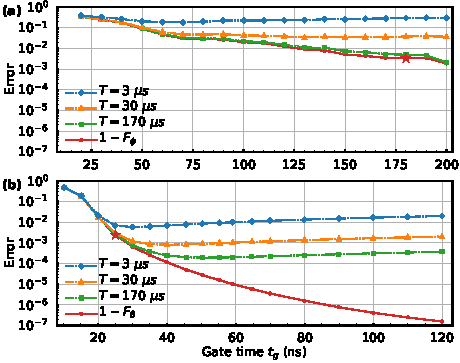
\includegraphics[width=\colfigwidth]{chapter-4-zero-pi/figs/xgate_fidelity.pdf}
\centering
\caption[Simulated $X$ gate error versus gate time.]{
Simulated $X$ gate error $1-F$ versus gate time $t_g$ for numerically optimized pulses driving (a) $n_\phi$ and (b) $n_\theta$.
Solid lines represent coherent gate error without added noise.
Dashed lines show the performance including open-system evolution with energy relaxation and pure dephasing, with $T_1=T_\phi=T\in\{3,30,170\}\,\mu\mathrm{s}$.
The two stars correspond to the pulses considered in \cref{zp:fig:xgate_phi} and \cref{zp:fig:xgate_theta}.
The simulations here use a reduced model with 160 levels for the $n_\phi$ gate and 157 levels for the $n_\theta$ gate.
See \cref{zp:app:1Qgate_simulation} for further numerical implementation details.
}\label{zp:fig:xgate_fidelity}
\end{figure}

\begin{table}[htbp]
\centering
\setlength{\tabcolsep}{3.5pt}
\renewcommand{\arraystretch}{1.2} % Adjust the value as needed
\resizebox{\textwidth}{!}{%
\begin{tabular}{ccccc ccccc cc }
\toprule
$n_{\rm op}$ & Intermediate & $ n_{ \rm op}^{ 0\text{-} i} $ & $n_{\rm op}^{ 2\text{-} i} $ & Leakage
& $t_g$ & $\Omega_{0\text{-}i}$  & $\Omega_{2\text{-}i}$  & $\delta_1$ & $\delta_2$ & $F_{\rm optimize}$ & $F_{\rm open}$   \\
& states &  &  & states & (ns) & ($2\pi\cdot$MHz)  & ($2\pi\cdot$MHz) & ($2\pi\cdot$MHz) & ($2\pi\cdot$MHz) &  & ($T$=30$\mu$s) \\
\midrule
$n_\phi$ & $\ket{9}$ & 0.049 & 0.020 & $[\ket{10}, \ket{19}, \ket{33} ]$  & 180.0 & 66.08 & 10.81 & 335.73 & 360.59 & 99.659\% & 96.183\%  \\
$n_\theta$ & $\ket{7}$ & 0.052 & 0.191 & $\ket{25}$ & 25.0  & 59.87 & 56.29  & -3.79  & 1.54   & 99.758\% & 99.713\% \\
\bottomrule
\end{tabular}}
\caption[Optimized $X$ gate parameters.]{
Numerically optimized parameters corresponding to the two highlighted red stars in \cref{zp:fig:xgate_fidelity}.
The drive amplitudes and detunings $A_i/2\pi,\ \delta_i/2\pi$ are limited to be less than $500$ MHz.
The effective Rabi rates are given by $\Omega_{0\text{-}i}=A_1(e^2-1)n_{\rm op}^{0\text{-}i}$ and $\Omega_{2\text{-}i}=A_2(e^2-1)n_{\rm op}^{2\text{-}i}$.
}
\label{zp:tab:xgate_parameters}
\end{table}

Charge dispersion is negligible at the chosen operating point [\cref{zp:fig:circuit_potential}(d)], so we include only flux-induced pure dephasing.
At $\phi_{\rm ext}=0$, the first-order flux sensitivity vanishes, and the dephasing rate is determined by the curvature of the transition frequency~\cite{hays2025nondegenerate},
\begin{align} \label{zp:eq:zp_tphi}
\frac{1}{T^\varphi_{0\text{-}l}} = A_{\phi_{\rm ext}} \left| \frac{\partial^2 \omega_{0\text{-}l}}{\partial \phi_{\rm ext}^2} \right|.
\end{align}
We choose $A_{\phi_{\rm ext}}$ such that $T^\varphi_{0\text{-}2}=T$, after which \cref{zp:eq:zp_tphi} determines the remaining dephasing times.
We use the $\ket{0}\leftrightarrow\ket{2}$ transition for this calibration because it has the largest flux curvature among the transitions in the effective $\Lambda$ system.

There are two key points to emphasize.
First, when we specify a noise strength such as $T = 3 \mu\text{s}$, we refer to both relaxation and dephasing times associated with the relevant transitions of the gate.
Second, for simplicity, we adopt a family of noise models in which relaxation and dephasing rates are equal, i.e., $T^r = T^\varphi = T$.

\subsection{Noisy gate fidelity vs. gate time} \label{zp:sec:fidelity_1q}
We evaluate gate performance using the average infidelity between the ideal $X$ gate and its noisy implementation $\tilde{X}$, denoted $1-F(X,\tilde{X})$~\cite{pedersen_fidelity_2007,Wood2015}.
For each gate duration $t_g$, we optimize the pulse ($A$, $\delta$) parameters to minimize $\log_{10}(1-F)$ in a closed quantum system.
For additional details, see \cref{zp:app:sec:model_reduce_1q,zp:app:sub_sec_pluse_opt}.

The optimization pipeline is as follows.
For each gate time $t_g$, we optimize the two amplitudes $A_{1,2}$ and detunings $\delta_{1,2}$ in the closed-system model.
The amplitudes are constrained to $A/2\pi\in[0,500)~\text{MHz}$, and the detunings $\delta=\omega_d-\omega_{i\text{-}j}$ are varied within $\pm\,2\pi\times500~\text{MHz}$ around the target transition $\omega_{i\text{-}j}$.
The gate error is then computed by applying pulses optimized in the closed-system model to the noisy evolution generated by the master equation in \cref{zp:eq:master_eq}.
For more details, see \cref{zp:app:sub_sec_pluse_opt,zp:app:sub_sec_noisy_1Q}.

\Cref{zp:fig:xgate_fidelity}(a) shows the simulated $X$-gate error $1-F$ versus gate time $t_g$ when driving $n_\phi$, while \cref{zp:fig:xgate_fidelity}(b) shows the corresponding results for driving $n_\theta$.
The $y$-axis scales are matched to enable direct comparison.
The key observation is that $X$ gates implemented via $n_\theta$ driving achieve both shorter gate times and higher fidelities than those obtained with $n_\phi$ driving.

There are two main reasons for this advantage.
First, in our parameter regime the relevant matrix elements of $n_\theta$ are significantly larger than those of $n_\phi$ (see \cref{zp:tab:xgate_parameters}).
In particular, $n_\theta^{2\text{-}7}/n_\phi^{2\text{-}9}\sim 10$ is an order of magnitude larger than $n_\theta^{0\text{-}7}/n_\phi^{0\text{-}9}\sim 1$.
Second, the $n_\theta$ drive has fewer leakage pathways than the $n_\phi$ drive, as seen in \cref{zp:fig:xgate_phi}(a)–(b) and \cref{zp:fig:xgate_theta}(a)–(b).
With fewer leakage channels, stronger and shorter drives can be used without compromising fidelity.
Moreover, the optimized drive frequencies for $n_\phi$ are often off-resonant (for the gate times considered), while those for $n_\theta$ are typically near-resonant, further reducing leakage.

The optimized gates are significantly faster than the experimentally demonstrated gate in Ref.~\cite{Gyenis_zero_pi_2021a}.
In \cref{zp:sec:x_gate_reproduce}, we give some explanation for this apparent discrepancy (e.g., experimental limitations on drive amplitude, mixed mode coupling, and decoherence not predicted by our phenomenological noise model).
Ultimately, we show that our numerical models can roughly reproduce the behavior observed in the experiment.

\section{ Coupling for Two \texorpdfstring{\zp}{zero pi} Qubits} \label{zp:sec:coupling}
Our single-qubit analysis shows that coupling to the $\theta$ mode provides larger charge matrix elements and fewer leakage pathways than coupling to the $\phi$ mode.
Motivated by this finding, we focus on designing two-qubit gates based on a charge-charge interaction between the two circuits' $\theta$ modes, i.e., an $n_{\theta1} n_{\theta2}$ interaction.

The $\theta$ mode involves all nodes of the \zps circuit, so producing an $n_{\theta1} n_{\theta2}$ interaction requires multi-node coupling.
We show two such schemes in \cref{zp:fig:circuit_2qubits}.
The Hamiltonian for these two \zps systems can be written as
\begin{align}\label{zp:eq:coupled_zp_ham}
     H_{\rm cp} =  H_{0\text{-}\pi}^{(1)} +  H_{0\text{-}\pi}^{(2)} +  H_{\rm int},
\end{align}
where the superscript $(i)$ refers to the $i$th qubit and $H_{\rm int}$ is the interaction Hamiltonian.
The two circuits in \cref{zp:fig:circuit_2qubits} (a) and (b) yield interactions
\begin{subequations}
\begin{align}
    H_{\rm int}^{\rm (a)} &= g_{\theta} n_{\theta1} n_{\theta2} ~, \\
    H_{\rm int}^{\rm (b)} & = g_{\theta} n_{\theta1} n_{\theta2} - g_{\phi} n_{\phi1} n_{\phi2} ~.
\end{align}
\end{subequations}
Circuit (a) implements a pure $n_{\theta1} n_{\theta2}$ interaction and forms the foundation of our two-qubit gate implementation.
Circuit (b) does not produce a pure  $n_{\theta1} n_{\theta2}$ interaction.
Nonetheless, circuit (b) does have some advantages despite its mixed interaction.
Notably, it requires fewer capacitors, making it easier to construct, and the renormalized $\tilde E_C^\phi$ remains light even with a large coupling capacitor.
A full derivation of both interactions is provided in \cref{zp:app:quantize}.
Since the remainder of the chapter focuses on circuit~(a), we briefly outline its derivation below.

\begin{figure}[htbp]
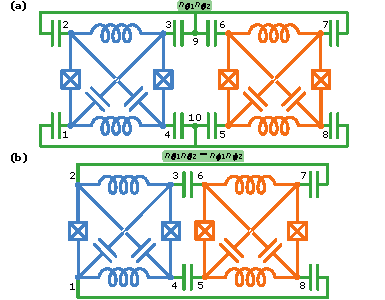
\includegraphics[width=\colfigwidth]{chapter-4-zero-pi/figs/circuit_2qubits.pdf}
\centering
\caption[Two capacitively coupled \zps qubits.]{
Two coupled \zps qubits with (a) pure $g_{\theta} n_{\theta1} n_{\theta2}$ and (b) mixed $g_{\theta} n_{\theta1} n_{\theta2} - g_{\phi} n_{\phi1} n_{\phi2}$ interaction terms.
The individual qubits are shown in blue and orange, while the coupling circuit is drawn in green.
}\label{zp:fig:circuit_2qubits}
\end{figure}

Because the coupling network in circuit~(a) is purely capacitive, it modifies only the kinetic terms in the Lagrangian.
As labeled in \cref{zp:fig:circuit_2qubits} (a), nodes 1–4 correspond to qubit 1, nodes 5–8 to qubit 2, and nodes 9–10 to the coupler.
With this convention, the interaction Lagrangian in node flux variables is
\begin{align} \label{zp:eq:zp_interact_theta_lagrangian_1}
T_{\rm{int}}=\frac{C_{c}}{2} \big [
&(\dot{\varphi }_1-\dot{\varphi }_{10}){}^2
+(\dot{\varphi }_4-\dot{\varphi }_{10}){}^2
+(\dot{\varphi }_5-\dot{\varphi }_{10}){}^2     \nonumber\\
&+(\dot{\varphi }_8-\dot{\varphi }_{10}){}^2
+(\dot{\varphi }_2-\dot{\varphi }_9){}^2
+(\dot{\varphi }_3-\dot{\varphi }_9){}^2        \nonumber\\
&+(\dot{\varphi }_6-\dot{\varphi }_9){}^2
+(\dot{\varphi }_7-\dot{\varphi }_9){}^2 \big ]   \,.
\end{align}
Here, $C_c$ is the value of the coupling capacitors, shown in green in \cref{zp:fig:circuit_2qubits}.
\Cref{zp:eq:zp_interact_theta_lagrangian_1} shows that both qubits couple to nodes 9 and 10.

After performing the variable transformation in \cref{zp:eq:zp_transform} and setting $\varphi_{\pm}=\varphi_9 \pm \varphi_{10}$, we obtain
\begin{align} \label{zp:eq:zp_interact_theta_lagrangian_2}
T_{\rm{int}}
=&\frac{C_c}{2}\sum_{i=1}^{2} \big [\dot{\phi}_i^2 + \dot{\zeta}_i^2
+(\dot{\varphi }_+ - \dot{\Sigma }_i)^2
+(\dot{\varphi }_- - \dot{\theta }_i)^2 \big ] \, .
\end{align}
The $\varphi_-$ mode is coupled directly to both $\theta_1$ and $\theta_2$.
There are no potential energy terms corresponding to the $\Sigma_1$, $\Sigma_2$, $\varphi_+$, and $\varphi_-$ modes, so they are ``free modes'' and can be removed from the Lagrangian \cite{groszkowskiScqubitsPythonPackage2021a,ding_free-mode_2021,chittaComputeraidedQuantizationNumerical2022a}.

After free mode removal and circuit quantization, the coupling Hamiltonian is
\begin{align} \label{zp:eq:zp_2_qubit_coupling_theta_2}
 H_{\rm{int}} =
g_\theta\, {n}_{\theta 1} {n}_{\theta 2} \, ,
\end{align}
with coupling energy
\begin{equation} \label{zp:eq:g_theta}
g_\theta =
\frac{2e^2C_c}{\tilde C_{\theta} (\tilde C_{\theta} - C_c)} \approx \frac{e^2C_c}{2C^2}\,.
\end{equation}
Here $\tilde C_{\theta}=2C + 2C_J +C_0 +C_c = C_{\theta} + C_c $.
The approximation is valid when $C\gg C_c, C_J, C_0$.

One consequence of capacitive coupling is the renormalization of each qubit’s charging energy.
For the circuit in \cref{zp:fig:circuit_2qubits} (a), the charging energies become
 \begin{align}
    \tilde E_C^\phi = \frac{e^2}{2 \tilde C_\phi} , \quad
    \tilde E_C^\theta = \frac{e^2(2 \tilde C_\theta-C_c)}{4
\tilde C_{\theta}( \tilde C_{\theta} - C_c)}
     \, ,
 \end{align}
where $\tilde C_\phi = 2 C_J +C_0 +C_c = C_\phi +C_c$.
The coupling capacitance makes both modes heavier ($\tilde E_C^\phi < E_C^\phi$ and $\tilde E_C^\theta  < E_C^\theta$), and these changes can be significant.
Using the parameters from \cref{zp:tab:parameter_zp}, $(C_J,C_0,C_c)\approx(2,13,19)\,\mathrm{fF}$, $\tilde E_C^\phi$ and $\tilde E_C^\theta$ decrease by approximately $50\%$ and $4\%$, respectively.
The hard \zps regime requires $E_L,E_C^\theta\ll E_C^\phi$.
This is difficult to achieve in circuit (a) because the coupling capacitance suppresses $E_C^\phi$.
Specifically, in a hard \zps regime, we expect $C_c\gg C_J$ and $C_0 \rightarrow 0$, so the $\phi$ mode charging energy scales with $\tilde E_C^\phi\propto 1/2C_c$.
Thus, a very large inductance and shunt capacitance would be required to achieve the hard \zps regime.
Circuit (b) avoids this limitation because $\tilde E_C^\phi \propto \left[1/C_J+1/(C_J+C_c)\right]$, which approaches $1/C_J$ when $C_c\gg C_J$.

The coupling schemes in \cref{zp:fig:circuit_2qubits} are experimentally demanding.
They require capacitive access to all four nodes of each \zps qubit, together with a multi-node coupling network and additional control and readout circuitry.
The resulting layout is substantially more complex than that of conventional superconducting-qubit architectures.
Suppressing parasitic capacitances remains an open challenge.
Our analysis also assumes identical circuit elements, for which unwanted coupling terms cancel exactly.
In a realistic device, disorder in the coupling capacitors and stray capacitances will break this symmetry and generate residual interactions.
We nevertheless adopt the zero-disorder limit because it reduces the Hilbert-space dimension, simplifies the numerical analysis, and establishes a best-case benchmark for gate performance.
A detailed treatment of disorder, parasitic couplings, and layout constraints is left for future work.

Before closing this section, we briefly comment on generalizations of this coupling scheme.
Similar layouts can be used to connect any pair of \zps modes, and we show the required connections in \cref{zp:tab:coupling_table}.
As with the system in \cref{zp:fig:circuit_2qubits} (a), these coupling circuits require many more capacitors than are typically needed in transmon architectures, even before accounting for drive lines.

\begin{table}[htbp]
\centering
\setlength{\tabcolsep}{7pt}
\renewcommand{\arraystretch}{1.05}
\begin{tabular}{ccc}
\toprule
\small
Interaction                    & Nodes coupled to 9        & Nodes coupled to 10     \\ \midrule
$n_{\theta 1}n_{\theta 2}$  & 2,3 + 6,7         & 1,4 + 5,8       \\
$n_{\phi 1}n_{\phi 2}$      & 1,3 + 5,7         & 2,4 + 6,8       \\
$n_{\theta 1}n_{\phi 2}$    & 2,3 + 5,7         & 1,4 + 6,8       \\
$n_{\phi 1}n_{\theta 2}$    & 1,3 + 6,7         & 2,4 + 5,8       \\ \bottomrule
\end{tabular}
\caption[Capacitive connections coupling \zps modes.]{
Capacitive connections that couple the specified modes of two \zps qubits.
Node numbers match \cref{zp:fig:circuit_2qubits} (a).
}\label{zp:tab:coupling_table}
\end{table}

\section{Microwave-activated CZ gate}\label{zp:sec:cz}
We now develop a CZ gate for two coupled \zps qubits, using the coupling scheme from \cref{zp:sec:coupling} and a microwave drive applied to one qubit.
Inspired by similar CZ and CCZ gates in fluxonium~\cite{nesterov2018microwave,ficheux2021fast,mazhorin2026nativecczgatefluxonium}, the gate drives a transition between a computational state and a higher non-computational state to accumulate a $\pi$ phase.
As in fluxonium, the \zps spectrum is crowded, necessitating careful consideration of competing transitions when optimizing gate performance.

\subsection{Driven Hamiltonian}\label{zp:sec_sub:cz_drive_params}
The Hamiltonian of the coupled qubits with drive is
\begin{align}\label{zp:eq:H_total_and_drive_cz}
    H_{\rm tot} = H_{0\text{-}\pi}^{(1)} + H_{0\text{-}\pi}^{(2)} +H_{\rm int} +H_{\rm drive}^{(2)},
\end{align}
where $H_{\rm drive}^{(2)}$ is a microwave drive on $n_{\theta 2}$ of the form given in \cref{zp:eq:zp_H_drive}.
The full circuit diagram is shown in  \cref{zp:fig:cz_ntheta}(a), with the drive circuitry highlighted in red.
It should be noted that the capacitive coupling to the voltage source induces additional energy renormalization, which we do not consider, as it is well studied in prior work~\cite{paolo_control_2019}.

We set device parameters so that both \zps circuits are in the soft regime, while allowing slight asymmetry.
The first qubit, described by $H_{0\text{-}\pi}^{(1)}$, uses the same parameters as the experimental device in Ref.~\cite{Gyenis_zero_pi_2021a}.
The second qubit, $H_{0\text{-}\pi}^{(2)}$, has $E_J$ reduced by 10\%, with all other parameters unchanged (see \cref{zp:tab:parameter_zp}).

To analyze the gate operation, we establish the following notation.
The eigenstates of the uncoupled system ($H_{\rm int} = 0$) are denoted $\ket{k,l}_0$, where $k$ and $l$ label the eigenstates of the first and second qubits, respectively.
These are commonly referred to as bare states.
With finite coupling ($H_{\rm int}\ne 0$), the ``dressed'' eigenstates are denoted $\ket{k,l}$ with eigenvalues $E_{k,l}$.
Each dressed state is indexed by the bare state with which it has the largest overlap.
For example, the dressed state $\ket{5,0}$ is defined by its large overlap with $\ket{5,0}_0$: $\left|{}_0\!\langle 5,0| 5,0 \rangle \right|=0.91$.
In addition, a key quantity is the transition frequency between dressed states.
For a transition $\ket{k,l}\text{-}\ket{k',l'}$, we denote the transition frequency as  $\omega_{k,l\text{-} k',l'} = |\omega_{k,l}-\omega_{k',l'}|$ with $\omega_{k,l}= E_{k,l}/\hbar$.

\subsection{Gate Concept and Transition Landscape}\label{zp:sec:cz_gate_transition}
A two-qubit gate requires an interaction between the two \zps circuits, as described by the total Hamiltonian in \cref{zp:eq:H_total_and_drive_cz}.
Because charge matrix elements within the logical subspace are strongly suppressed, direct microwave-driven transitions between logical states are impractical.
To overcome this limitation, we use $H_{\rm drive}^{(2)}$ to drive a transition between a logical state and a non-computational state, thereby avoiding direct population transfer within the logical subspace.

Many CPHASE-gate schemes selectively couple the computational state $\ket{1,1}_L$ to a non-computational auxiliary state, e.g.,  $\ket{2,0}$ for a transmon.
The drive returns the population to $\ket{1,1}_L$ along a closed trajectory on the corresponding Bloch sphere.
This cyclic evolution gives $\ket{1,1}_L$ a geometric phase relative to the other computational states, set by the solid angle enclosed by the trajectory~\cite{nesterov2018microwave,ficheux2021fast}.
A complete resonant round trip produces a phase of $\pi$ and therefore implements a CZ gate.
Closed trajectories that enclose a smaller solid angle produce a smaller controlled phase.

Our two-qubit gates exploit the static qubit--qubit interaction $H_{\rm int}$ to lift the degeneracy of otherwise identical transition frequencies, while $H_{\rm drive}^{(2)}$ selectively drives one of the resulting transitions.
For two coupled quantum systems, as the interaction strength $g$ is increased from 0, degenerate states hybridize if they are coupled by the interaction.
The hybridization gap grows with the magnitude of the matrix element $\left|{}_0\bra{n',m'} H_{\rm int} \ket{n,m}_0\right|$.
Corresponding transitions in the dressed basis are split.
This splitting enables gates that selectively drive one of the previously degenerate transitions.\footnote{There is no direct coupling between logical states in the \zp, so the static $ZZ$ rate $(\omega_{0,2-2,2} - \omega_{0,0-2,0})/2\pi = \Gamma_{\rm ZZ}=171$ Hz of the coupled \zps system is substantially smaller than in transmon or fluxonium devices with comparable interaction strength.}

\begin{figure}[htbp]
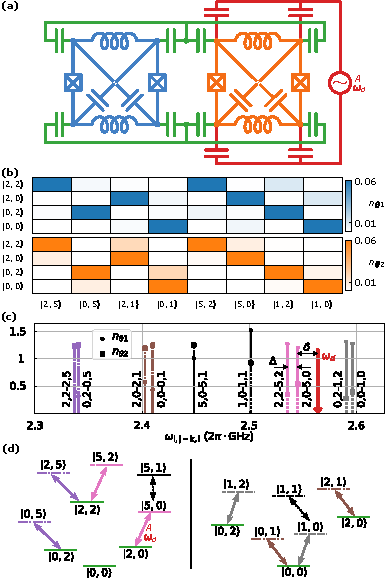
\includegraphics[width=\colfigwidth]{chapter-4-zero-pi/figs/cz_ntheta.pdf}
\centering
\caption[CZ gate implemented by driving $n_{\theta 2}$.]{
CZ gate implemented by driving $n_{\theta 2}$.
(a) Circuit diagram.
The coupling and drive circuits are depicted in green and red, respectively.
(b) Dressed basis charge matrix elements $\bra{i,j}n_{\theta r}\ket{k,l}$ for $r\in \{1, 2\}$.
The matrix elements are between two-qubit logical states (y-axis) and some non-logical states (x-axis).
Four pairs of dominant matrix elements are present in both diagrams.
(c) Charge matrix elements $\bra{i,j}n_{\theta r}\ket{k,l}$ for $r\in \{1, 2\}$ versus transition frequency $\omega_{i,j\text{-}k,l}$.
Solid lines ending in circles denote $n_{\theta 1}$, and dashed lines ending in squares denote $n_{\theta 2}$.
(d) Energy level diagram.
Four transition pairs in the CZ gate are denoted by solid arrows, using the same color scheme as in (c).
Other leakage transitions are represented by dashed arrows.
}\label{zp:fig:cz_ntheta}
\end{figure}

We now identify a suitable transition for implementing the CZ gate.
In the case of \zp, the interaction Hamiltonian most strongly couples states involving the logical states and the $\ket{1}$ and $\ket{5}$ non-computational states.
As a result, four prominent pairs of conditionally split transitions emerge, which we show in \cref{zp:fig:cz_ntheta} (c) and (d):
\begin{itemize}
\item pink pair: $\ket{2,0}\leftrightarrow\ket{5,0}$ and $\ket{2,2}\leftrightarrow\ket{5,2}$,
\item  gray pair: $\ket{0,0}\leftrightarrow\ket{1,0}$ and $\ket{0,2}\leftrightarrow\ket{1,2}$,
\item purple pair: $\ket{0,2}\leftrightarrow\ket{0,5}$ and $\ket{2,2}\leftrightarrow\ket{2,5}$,
\item brown pair: $\ket{0,0}\leftrightarrow\ket{0,1}$ and $\ket{2,0}\leftrightarrow\ket{2,1}$.
\end{itemize}
Recall that the physical state $\ket{2}$ is our logical $\ket{1}_L$.
Only the transition $\ket{2,2}\leftrightarrow\ket{2,5}$ is analogous to the $\ket{1,1}_L \leftrightarrow \ket{2,0}$ transition used in a transmon CZ.
However, all such transitions result in a gate equivalent to a controlled-phase gate up to local single-qubit rotations.

To find the most suitable candidate, we additionally consider the frequency mismatch $\Delta$, defined as the frequency difference between the two transitions within each pair.
We expect that the most spectrally isolated transition will be the easiest to selectively drive.
Among the four pairs, the pair $[\ket{2,2} \text{-} \ket{5,2}, \ket{2,0} \text{-} \ket{5,0}]$ has the largest $\Delta = | \omega_{2,0 \text{-} 5,0} - \omega_{2,2 \text{-} 5,2} |$.

The matrix elements of these transitions depend strongly on which qubit is driven.
Transitions that primarily change the state of the first qubit, such as $\ket{2,0}\leftrightarrow\ket{5,0}$, have smaller matrix elements under an $n_{\theta2}$ drive than under an $n_{\theta1}$ drive.
This behavior is illustrated in \cref{zp:fig:cz_ntheta}(c).
For the selected pair, the $\ket{2,0}\leftrightarrow\ket{5,0}$ transition is sufficiently strong, whereas its conditional counterpart $\ket{2,2}\leftrightarrow\ket{5,2}$ is weaker.
The resulting matrix element asymmetry is greater than for an $n_{\theta1}$ drive, making this transition pair well suited for selective excitation.
We therefore choose $\ket{2,0}\leftrightarrow\ket{5,0}$ as the primary driven transition under an $n_{\theta2}$ drive.
The combination of a large conditional frequency splitting, an appreciable target matrix element, and a strong matrix element asymmetry makes this transition the most favorable choice for implementing the CZ gate.

In practice, we use the selected transition frequency as a starting point and numerically optimize pulse parameters to maximize gate fidelity.
As seen in \cref{zp:fig:cz_population}, the optimized drive activates multiple transitions, rather than simply driving a round trip between $\ket{2,0}$ and $\ket {5,0}$.
It is possible to recover this simpler scheme at the cost of increased gate time.
Regardless of the intermediate populations, the final ``candidate'' gate is approximately diagonal in the computational basis and has the form
\begin{equation}\label{zp:eq:CZ_with_local_phases}
U_{\rm can} =  \mathrm{diag}\left[ e^{i \phi_{0,0}}, e^{i \phi_{0,2}}, e^{i \phi_{2,0}}, e^{i \phi_{2,2}}\right]\,.
\end{equation}
To arrive at the standard $ \text{CZ} =\mathrm{diag}[1,1,1,-1]$ gate, we apply single-qubit $z$ rotations  $R_z(\phi)=\exp[-i \phi Z/2] $ to \cref{zp:eq:CZ_with_local_phases}.
In particular, we transform $U_{\rm can} $ to  $U_{\rm std} = \left[ R_z(\alpha_2) \otimes R_z(\alpha_1) \right] U_{\rm can} $, where $\alpha_1 = \phi_{0,0}-\phi_{0,2}$ and $\alpha_2 = \phi_{0,0}-\phi_{2,0}$ cancel the local phases.
When applying these phase corrections to $U_{\rm can}$, we arrive at
\begin{equation}
U_{\rm std} = e^{i \phi_g}\mathrm{diag} \left[ 1, 1, 1, e^{i\chi} \right] \, .
\end{equation}
Here, $\phi_g= (\phi_{0,2} +\phi_{2,0})/2$ is a global phase, and $\chi = \phi_{2,2}+ \phi_{0,0} - \phi_{0,2}- \phi_{2,0}$ is the controlled phase.
For an ideal CZ gate, $\chi=\pi$.

We now briefly discuss an alternative drive scheme that results in a CNOT gate.
This CNOT gate uses a two-qubit $\Lambda$-type transition, inspired by the single-qubit $X$ gates in \cref{zp:sec:1q}.
Thus it requires a two tone drive on one of the qubits.
Full details are provided in \cref{zp:sec:cnot}.
In noiseless simulations, the CNOT gate achieves fidelities above $99.9\%$, but it is about two times slower than the CZ gate at comparable fidelities.
The slower operation results from the weaker transition matrix elements and smaller conditional frequency splittings involved.
This CNOT construction serves as a proof of principle that the coupling architecture supports microwave-activated two-qubit gates beyond the CZ gate.

\section{CZ Gate Performance with Decoherence} \label{zp:sec:fidelity_2q}
In this section, we present numerically optimized CZ pulses.
We additionally extend the single-qubit noise model presented in \cref{zp:sec:noise_1q} to two coupled qubits and examine the optimized pulses subject to this noise model.
Performing these open-system simulations is computationally intensive and requires careful construction of the two-qubit Hamiltonian.
We refer the interested reader to \cref{zp:sec:2Qgate_simulation} for additional numerical details.

\begin{table}[htbp]
\centering
\setlength{\tabcolsep}{3.5pt}
\renewcommand{\arraystretch}{1.2} % Adjust the value as needed
\resizebox{\textwidth}{!}{%
\begin{tabular}{cccc ccc cc}
\toprule
Gate & $n_{\rm op}$ & Transitions & Associated $n_{\rm op}$ & $t_g$ & $\Omega_1$   & $\delta_1$  & $F_{\rm optimize}$ & $F_{\rm open}$  \\
 &  &  &  & (ns) & ($2\pi\cdot$MHz)  & ($2\pi\cdot$MHz)  &  & ($T=30~\mu\mathrm{s}$) \\
\midrule
\multirow{2}{*}{CZ} & \multirow{2}{*}{$n_{\theta 2}$} & \multirow{2}{*}{$\ket{2,0}$-$\ket{5,0}$} & \multirow{2}{*}{$0.537$} & 91.95 & 61.45  & 25.19  & 99.893\% & 99.830\%  \\
 &  &  &  & 182.01 & 27.04  & 13.13  & 99.993\% & 99.908\%  \\
\bottomrule
\end{tabular}}
\caption[Optimized CZ pulse parameters.]{
The parameters of the two CZ pulses corresponding to the red star and pentagon in \cref{zp:fig:2q_fidelity}.
$A_i/2\pi$
is limited to be less than $250$ MHz.
The effective Rabi rate is given by $\Omega_{1}=A_1(e^2-1)n_{\rm op}$.
}\label{zp:tab:parameter_cz}
\end{table}

\subsection{Two-Qubit Noise Model}\label{zp:sec:noise_2q}

Our phenomenological two-qubit noise model is built as a tensor product of independent single-qubit noise channels.
Let $L^r_{ij}$ and $L^\varphi_l$ denote single-qubit relaxation and dephasing Lindblad operators from \cref{zp:eq:lindblad_ops}.
The two-qubit operators are constructed as
\begin{equation}
\mathfrak{L}^{(1)} = L \otimes I\,\, {\rm and} \,\, \mathfrak{L}^{(2)} = I \otimes L\,,
\end{equation}
with $L \in \{L^r_{ij},\, L^\varphi_l\}$.
Though each operator requires multiple indices to characterize the noise process, here we omit them for clarity.
The decay and dephasing rates are chosen as in the single-qubit case (see \cref{zp:sec:noise_1q}).
In particular, we choose $T_1= T_\phi=T$ for both qubits.
Dynamics are simulated using the master equation in \cref{zp:eq:master_eq}.
The full two-qubit state is evolved to obtain a propagator and gate fidelity.
We provide a more thorough description of the open-system model in \cref{zp:app:subsec_2Q_noise_details_and_converge}.

\subsection{Optimized Gate}\label{zp:sec:2q_gate}

\begin{figure}[htbp]
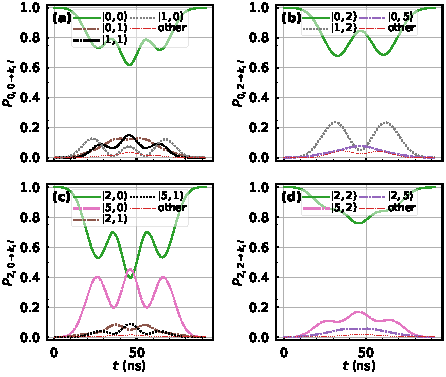
\includegraphics[width=\colfigwidth]{chapter-4-zero-pi/figs/cz_population_tg=91.pdf}
\centering
\caption[Population transfer during the CZ gate.]{Noiseless simulation of population transfer during a CZ gate at $t_{\rm g}=91.95$ ns with $F=99.893\%$.
$P_{i,j \text{-} k,l }$ denotes the population of state $\ket{k,l}$ for an initial state $\ket{i,j}$.
The initial states in panels (a)--(d) are $\ket{0,0}$, $\ket{0,2}$, $\ket{2,0}$, and  $\ket{2,2}$, respectively.
The ``other'' state refers to the total population of all states not explicitly shown within the lowest 1000 dressed states.
}\label{zp:fig:cz_population}
\end{figure}

To understand the gate mechanism, we examine the noiseless population dynamics during an optimized CZ gate.
In \cref{zp:fig:cz_population}, we show these dynamics for a gate with $t_g = 91.95$~ns and $F= 99.893\%$.
The gate uses a single Gaussian pulse to simultaneously drive multiple transitions.
The main CZ transition $\ket{2,0}\text{-}\ket{5,0}$, shown in panel (c), reaches approximately   $40\%$ population in $\ket{5,0}$.
Additional non-computational states associated with the four identified transition pairs are also appreciably populated.
For example, \cref{zp:fig:cz_population}(d) shows population transfer from $\ket{2,2}$ to both $\ket{2,5}$ and $\ket{5,2}$.
Despite the nontrivial intermediate dynamics, leakage is small at the end of the gate, with the final population in all other states below $0.4\%$.
These excursions are acceptable under the noise model considered in \cref{zp:sec:noise_2q}, although intermediate populations can be reduced by increasing the gate duration or utilizing smaller controlled-phase operations.

\begin{figure}[htbp]
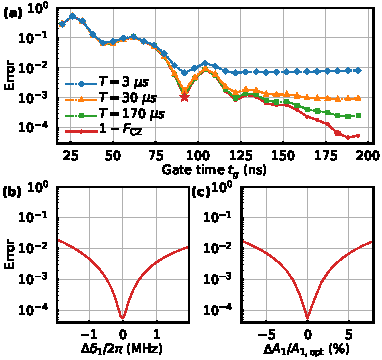
\includegraphics[width=\colfigwidth]{chapter-4-zero-pi/figs/cz_fidelity.pdf}
\centering
\caption[CZ gate performance.]{
CZ gate performance.
(a) Gate error ($1-F$) versus gate time $t_g$, using optimized pulse parameters for each $t_g$.
Solid lines show errors for unitary (closed-system) evolution, while dashed lines include decoherence with $T_1=T_\phi=T\in\{3,30,170\}\,\mu\mathrm{s}$.
The star marks the operating point illustrated in \cref{zp:fig:cz_population}.
We use a reduced model with 60 states to simulate this gate.
See \cref{zp:app:subsec_2Q_noise_details_and_converge} for additional modeling details.
(b) Coherent gate error as a function of the drive-detuning deviation $\Delta\delta_1=\delta_1-\delta_{1,\mathrm{opt}}$ at $t_g=182$ ns, with the drive amplitude fixed at its optimized value.
(c) Coherent gate error as a function of the relative drive-amplitude deviation $\Delta A_1/A_{\mathrm{opt}}=(A_1-A_{1,\mathrm{opt}})/A_{1,\mathrm{opt}}$ at $t_g=182$ ns, with the detuning fixed at its optimized value.
Full pulse parameters for both highlighted pulses are given in \cref{zp:tab:parameter_cz}.
}\label{zp:fig:2q_fidelity}
\end{figure}

\Cref{zp:fig:2q_fidelity} shows how the gate error $1-F$ scales with gate time $t_g$ for the CZ gate under different coherence times.
Panel (a) clearly shows that the CZ gate is coherence limited for shorter lifetimes.
For $T=3\,\mu\mathrm{s}$, for example, the minimum error is approximately $10^{-2}$, whereas for $T=30\,\mu\mathrm{s}$ it reaches approximately $10^{-3}$.
Within our phenomenological noise model, the dominant error arises from dephasing of the logical state $\ket{1}_L=\ket{2}$.
Panels (b) and (c) show the coherent gate-error landscapes near the optimized operating point as the drive detuning and amplitude are varied.
This allows us to assess the robustness of gates to control-parameter errors.
The coherent fidelity remains above $99.9\%$ for drive-frequency deviations of approximately $500$ kHz and drive-amplitude deviations of about $\pm2\%$.
The resulting coherent errors are much smaller than those introduced by dissipation, indicating that the gate is reasonably robust to calibration errors.
For experimentally relevant coherence times, fidelity is therefore limited by logical-qubit coherence, rather than by coherent control errors.

Finally, we investigate the robustness of the optimized CZ gate to device-fabrication imperfections.
We independently vary each circuit parameter of the second qubit by up to $\pm5\%$, re-optimize the gate, and compute the resulting infidelity.
The results, summarized in \cref{zp:app:sensitivity}, show that the gate is most sensitive to variations in $E_{C}$, $E_{L}$, and $E_{J}$, but relatively insensitive to changes in $\phi_{\mathrm{ext}}$, $n_{g}^\theta$, $E_{Cc}$, $E_{CJ}$, and $E_{C0}$.
Nevertheless, the median degradation in gate performance is small over the parameter ranges considered, particularly for longer gate times.

\section{Conclusion}\label{zp:sec:conc}

In summary, we have proposed and analyzed a two-qubit CZ gate for capacitively coupled soft \zps circuits.
Using a phenomenological noise model, we find that modest improvements in experimental coherence times to the tens-of-microseconds regime could enable the CZ gate to achieve error rates of approximately $10^{-3}$.
These results position the soft \zps as a promising intermediate platform between conventional superconducting qubits and more strongly protected qubits.

To make our numerical modeling tractable, we made several simplifying assumptions.
Our analysis and simulations assume zero-disorder and neglect the $\zeta$ mode, neither of which is realistic.
We also model decoherence phenomenologically rather than through a microscopic description of the device environment.
These approximations are sufficient to establish the feasibility of the proposed gate protocols, but the resulting fidelities should be interpreted as an upper bound, rather than as a quantitative prediction for a specific experimental device.
Moving beyond these approximations is numerically demanding but would be a worthwhile direction for future work.

Looking forward, several important directions are worth pursuing.
First, future theoretical work should quantify how disorder and additional harmonic modes, such as the $\zeta$ mode, affect gate performance.
Second, experimental measurements of relaxation and dephasing in higher-energy \zps states would enable more realistic noise models and pulse optimization.
Third, the performance of our gate as devices approach the hard-\zps regime is unclear.
Recent work by \citet{kolesnikowProtectedPhaseGate2026} has proposed protected single- and two-qubit gates for hard-\zps devices; incorporating realistic noise into that framework would be a  valuable next step.
